%Template file for Scientific Computation project 1 discussion and figures
\documentclass{article}
\usepackage[a4paper, margin=1in]{geometry}
\title{Scientific Computation Project 1 template}

\author{\emph{Nicholas Siedlaczek - 01533315}}

\usepackage{graphicx}

\begin{document}

\maketitle

%---------------- Part 1  -------------------
\hrule
\hrule

\section*{Question 1}


\subsection*{1(a)}
%Place your discussion for question 1(a) here}
The function \emph{code1} takes primary inputs L (a list of integers sorted into non-decreasing order) and x (an integer to attempt to find in this list). Furthermore indices can be chosen for the location in this list that the search should be limited to i.e. the function will try to find x in L[istart:iend]. If istart and iend are not specified then these will be chosen such that the entire list is searched. (Note also that if istart$>$iend the program will return -1000) \\ \\
 The function will then proceed with a pseudo-binary search (note this could happen 0 times depending on parameters) until the length of the sublist under consideration is less than input N0. Once this has happened a linear search will be performed on said sublist. Once element matching x has been found the function will return the index of this element. If there does not exist an element matching x in the list, the function will return -1000. \\\\
The implementation of this function is done recursively.
\subsection*{1(b)}
%Place your discussion for question 1(b) here
To analyse \emph{code1} we observe that the 'setup' section runs in constant time(comparisons, checks and potential assignments of integers).\\ \\
The check of iend-istart $<N_0$ is also constant time. We then consider the 'binary split' portion which will repeatedly run until iend-istart i.e. the length of the sublist is less than $N_0$, which will take $\log(N/N_0)$ evaluations of this 'fork' of the function, which only contains operations which have constant time, and hence has $O(\log(N/N_0))$ time. \\ \\
Once the 'sublist length' is less than $N_0$ we will perform a linear search of this 'sublist' which is well known to have $O(N_0)$ time. Combining everything we have that a worst case time complexity of code1 is $O(\log(\frac{N}{N_0}) + N_0)$
\subsection*{Figures}
\begin{figure}[h!]
\centering
%Uncomment line below to display figure saved as fig11.png
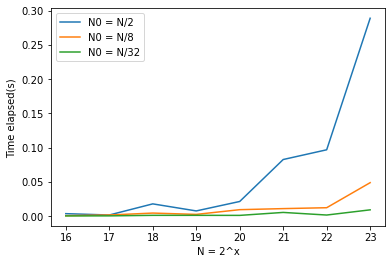
\includegraphics[width=0.9\textwidth]{code1.png}
\caption{Figure for question 1}
\label{fig1}
\end{figure}

Examining the figure we can see that increasing the size N of the list L inputted to 'code1' while keeping $N_0$ constant makes the time taken for the code to run increase(as evidenced by each sepearte line in the figure).
\\ \\Furthermore we can see that if N is kept constant and we increase the value of $N_0$(in relation to the size of N) we can see that it takes significantly longer for higher values of $N_0$. Both these facts seen in the figure can be seen from looking at the theoretical time complexity of code1).

%---------------- End Question 1 -------------------

\vspace{0.25in}

%---------------- Question 2  -------------------
\section*{Question 2}


\subsection*{2(b)}
My approach to the function findAA is as follows:
\begin{enumerate}
\item Convert the list of sequences of codons $L\_p$ into a list of sequences of amino acids, using function codon2AA
\item Convert the list of sequences of amino acids to a list of lists containing the base-20 representation of these amino acids, using function char2base20.
\item Use the Rabin-Karp algorithm to find occurences of the amino acid sequences corresponding to the sequences of codons contained in list $L\_p$ using function gene\_RK. If one of the codons in the input does not correspond to a gene, we give [-1000] as the output for that entry. Also if no occurences are found then we will return an empty list for that entry.
\end{enumerate}
Further information on my implementation can be found in docstrings on the functions and comments throughout.\\

Step 1 converts the p length 3m elements of $L\_p$ into p length m amino acid sequences. Each of these p elements contains m lookups from table T along with m asignments to list. This results in O(m) time, and doing this p times results in O(mp) time. \\

Step 2 converts the p length m amino acid sequences into base20. This involves m lookups assignments which each have constant time, and again there are p of these to do, therefore this step also has O(mp) time complexity. \\

Step 3 (i.e. the Rabin Karp algorithm) has a worst case complexity of O(mn) as each individual step has constant time, of which we do n times, giving O(n) complexity. The trouble is with the possibility of hash collistions(of which theoretically there should be low probability of). However assuming the worst case gives us the previously mentioned O(nm) complexity, again we do this on each of p elements giving a complexity of O(nmp). \\

Stringing these steps together in sequence will result in O($mp \cdot mp \cdot nmp$) = O($m^{3}p^{3}n$) time. Note in the average case the performance will be much better than this. We have used the most efficient method on each stage so overall we should expect it to also be efficient overall as there are no 'shortcuts' available.





%---------------- End Question 2 -------------------


\hrule
\hrule



%---------------- End document -------------------


\end{document}
